\documentclass[11pt]{article}
\renewcommand{\baselinestretch}{1.20} 
\usepackage[utf8]{inputenc}
\usepackage[english]{babel}
\usepackage{graphicx}
\usepackage{wrapfig}
\usepackage{subcaption}
\usepackage{geometry}
 \geometry{
  a4paper,
  total={170mm,237mm},
  left=20mm,
  top=30mm,
 }
 
\setlength{\abovecaptionskip}{15pt plus 3pt minus 2pt}

\rhead{Social hidden Messages 2018}
\lhead{Gruppe: B-125}
\chead{P2 - Rapport}
\rfoot{Page \thepage}

\title{Interaktions Design}
\author{ }
\date{ }

\begin{document}

\section{Positioning Tables and Figures}

\begin{figure}[!h]
    \begin{subfigure}[t]{0.5\textwidth}
        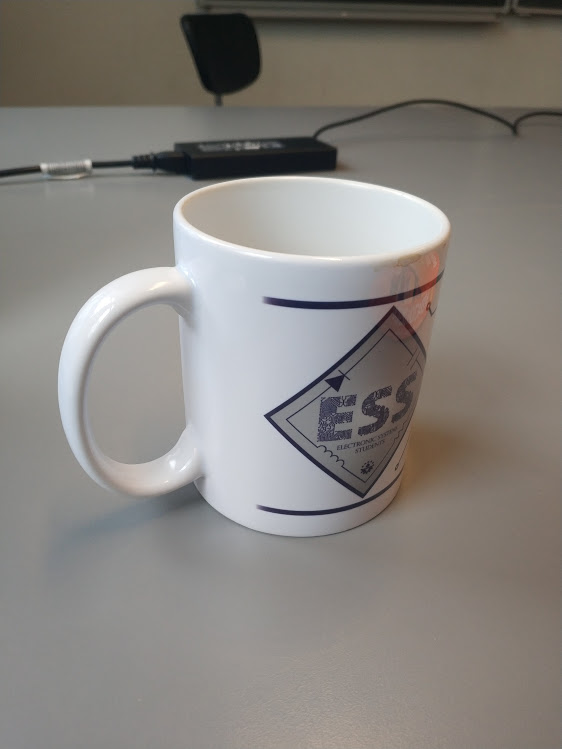
\includegraphics[scale=0.4]{InteraktionsDesign/Assets/kop.jpg}
        \caption{The cup has a great usability in that its easy to learn how to use it properly. The tap on the cup stands out from the otherwise cylinder shaped cup, which makes it very recognisable. The tap the cup has multiple purposes usability-wise, for instance it makes it safer to use when the cup contains hot liquid. The tap also makes for added efficiency and overall convenience.
        Moreover, the tap is shaped in such a way that it accommodates several fingers allowing for a solid grip with a range of hand sizes. The smooth finish of the handle is used for a pleasant user experience. The sense of control over the cup also adds to this pleasantness of the experience}
        \label{fig:cup}
    \end{subfigure}
    \begin{subfigure}[t]{0.5\textwidth}
        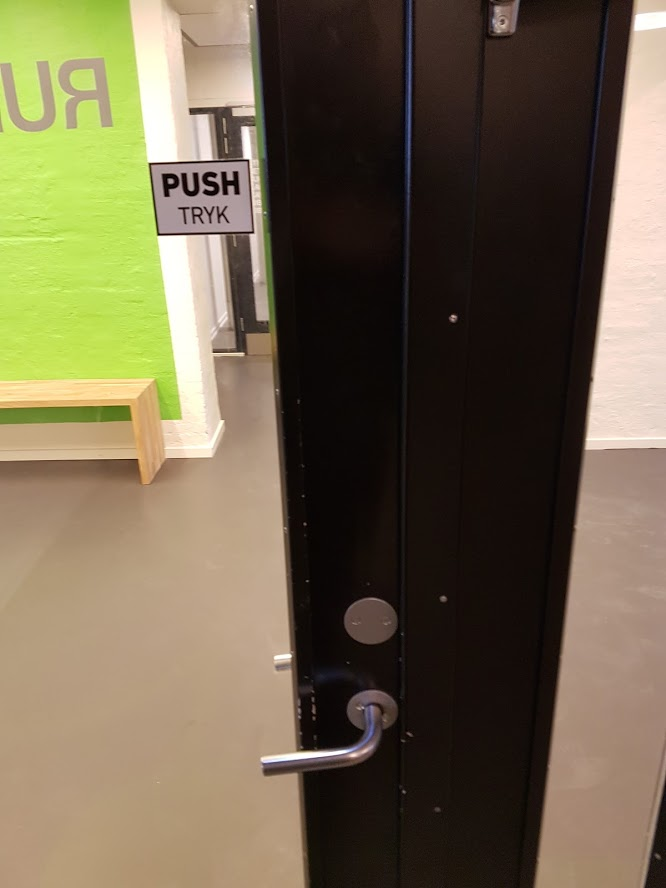
\includegraphics[scale=0.4]{InteraktionsDesign/Assets/door.jpg}
        \caption{The cup has a great usability in that its easy to learn how to use it properly. The tap on the cup stands out from the otherwise cylinder shaped cup, which makes it very recognisable. The tap the cup has multiple purposes usability-wise, for instance it makes it safer to use when the cup contains hot liquid. The tap also makes for added efficiency and overall convenience.}
        \label{fig:cup}
    \end{subfigure}
\end{figure}

\newpage

\section{Questionnaire}

In this section we are expecting that our product is a app, used to send and receive hidden messages through Instagram. This is done by letting the user select a forum "subject", and then post answers or new questions through a written message. The app then hides the message in a picture, and posts it on Instagram for everybody to see. The app then also contains functionality to receive and decrypt these messages again, to display for other users.\\
The Goal with this questionnaire is to identify the applications user group. This is so that the group has an easier time creating a good design platform, wanted by the users.\\\\
\noindent
The group has discussed creating a questionnaire like the following.
The idea is that the questionnaire contains normal questions to define a specific user group.
But also questions that in a certain combination can be identified as typical users for our product.\\\\
\noindent
Users behavior survey:
\begin{enumerate}
    \item What is your age ?                                        [        ]
    \item What is your occupation, and for how many years ?         [Please Write:]

    \begin{left}
        \rule{0.5\textwidth}{.4pt}
    \end{left}
    \begin{left}
        \rule{0.5\textwidth}{.4pt}
    \end{left}\\\\
    \begin{left}
        \rule{0.5\textwidth}{.4pt}
    \end{left}
    \begin{left}
        \rule{0.5\textwidth}{.4pt}
    \end{left}

    \item How often do you use a computer ?                         [Never / Sometimes / Every day]
    \item What do you use your computer for ? (Multiple)
    \begin{itemize}
        \item Homebankning [ ]
        \item Work [ ]
        \item School [ ]
        \item Entertainment [ ]
        \item Social networking [ ]
        \item Shopping [ ]
        \item Others    [Please Write:]
    \end{itemize}
    
    \begin{left}
        \rule{0.5\textwidth}{.4pt}
    \end{left}
    \begin{left}
        \rule{0.5\textwidth}{.4pt}
    \end{left}\\\\
    \begin{left}
        \rule{0.5\textwidth}{.4pt}
    \end{left}
    \begin{left}
        \rule{0.5\textwidth}{.4pt}
    \end{left}
    
    \newpage
    
    \item Do you use any social media or forums ?                   [Yes / No]
    \item If yes what media do you use ? (Multiple)
    \begin{itemize}
        \item Facebook  [ ]
        \item Instagram [ ]
        \item Twitter   [ ]
        \item Reddit    [ ]
        \item Others    [Please Write:]
    \end{itemize}
    
    \begin{left}
        \rule{0.5\textwidth}{.4pt}
    \end{left}
    \begin{left}
        \rule{0.5\textwidth}{.4pt}
    \end{left}\\\\
    \begin{left}
        \rule{0.5\textwidth}{.4pt}
    \end{left}
    \begin{left}
        \rule{0.5\textwidth}{.4pt}
    \end{left}
    
    \item Do you feel that you have to act a certain way on social medial, that differs from your normal behaviors ?                                          [Yes / No]
    \item If Yes, Why ?                                         [Please Write]
    
    \begin{left}
        \rule{0.5\textwidth}{.4pt}
    \end{left}
    \begin{left}
        \rule{0.5\textwidth}{.4pt}
    \end{left}\\\\
    \begin{left}
        \rule{0.5\textwidth}{.4pt}
    \end{left}
    \begin{left}
        \rule{0.5\textwidth}{.4pt}
    \end{left}
    
    \item How much do you feel that your Privacy is perserved on the internet \\
    .[Not at all / To a point of satisfaction / Totally Perserved]
    \item Do you try to enhance your privacy, on the internet ? [Yes / No]
    \item If yes, how ?                                         [Please write]
    
    \begin{left}
        \rule{0.5\textwidth}{.4pt}
    \end{left}
    \begin{left}
        \rule{0.5\textwidth}{.4pt}
    \end{left}\\\\
    \begin{left}
        \rule{0.5\textwidth}{.4pt}
    \end{left}
    \begin{left}
        \rule{0.5\textwidth}{.4pt}
    \end{left}
    
\end{enumerate}

\end{document}